%------------------------ Packages ------------------------
\documentclass[12pt,a4paper]{article}
\usepackage[latin1]{inputenc}
\usepackage[T1]{fontenc}
\usepackage[pdftex]{graphicx}
\usepackage{float}
\usepackage{amsmath}
\usepackage{amssymb}
\usepackage[FIGTOPCAP]{subfigure}
\usepackage{color}
\usepackage[hidelinks]{hyperref}

\newcommand{\version}{\IfFileExists{../../version.txt}
{\input{../../version.txt}}
{\input{../../../version.txt}}
}

\newcommand{\command}[1]{%
\indent \fcolorbox{black}{white}{%
   \begin{minipage}{\dimexpr\textwidth-\parindent\relax}%
      #1
   \end{minipage}%
}
}

\newsavebox{\FVerbBox}
\newenvironment{sample}
{\par \vspace{0.2cm} \begin{lrbox}{\FVerbBox}
\begin{minipage}{\dimexpr\textwidth-\parindent\relax}}
{\end{minipage}
\end{lrbox}
\fcolorbox{black}{lightgray}{\usebox{\FVerbBox}}
\vspace{0.2cm}}

\newenvironment{sampletitle}
{\vspace{0.2cm} \noindent\textbf{Example} :
\begin{sample}}
{\end{sample}}

\newcommand{\samplecomment}[1]{%

\textit{#1}
}

\newcommand{\seealso}[1]{\vspace{0.2cm} \noindent\textbf{See also} :\par #1}

% tikz
\usetikzlibrary{calc}
\usetikzlibrary{arrows}
\usetikzlibrary{shadows}

\tikzset{block/.style={draw, text centered, fill=gray!10,drop shadow}}
\tikzset{connect/.style={draw, line width=1 pt}}

\begin{document}

\begin{center}
\textbf{\huge  \underline{Median filter}}
\end{center}
\vspace{0.5cm}


In image processing, it is often desirable to reduce noise from an image corrupted by defected pixels. One of the severals techniques is to use the Median filter. It is a nonlinear filter. \\


\begin{figure}[h!]
\centering
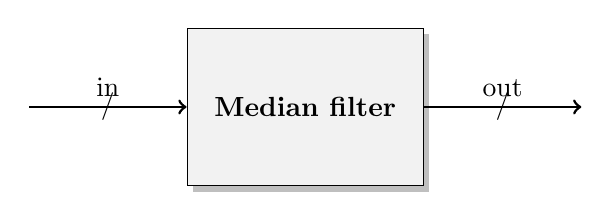
\begin{tikzpicture}
\node[block,rectangle,minimum height=2cm,minimum width=3cm] (bloc) {\textbf{Median filter}};

\path[connect,<-] ([yshift=0.0cm]bloc.west) -- node{/} node[above]{in} ++(-2cm,0);

\path[connect,->] ([yshift=0.0cm]bloc.east) -- node{/} node[above]{out} ++(2cm,0);
 ([xshift=0.5cm,yshift=-0.6cm]bloc.north);

\end{tikzpicture}
\end{figure}

\vspace{0.5cm}

Some examples with a noised initial image and the treathed image by a 1-stage median filter and then by a 2-stage median filter. \\

\begin{figure}[!h]
\centering
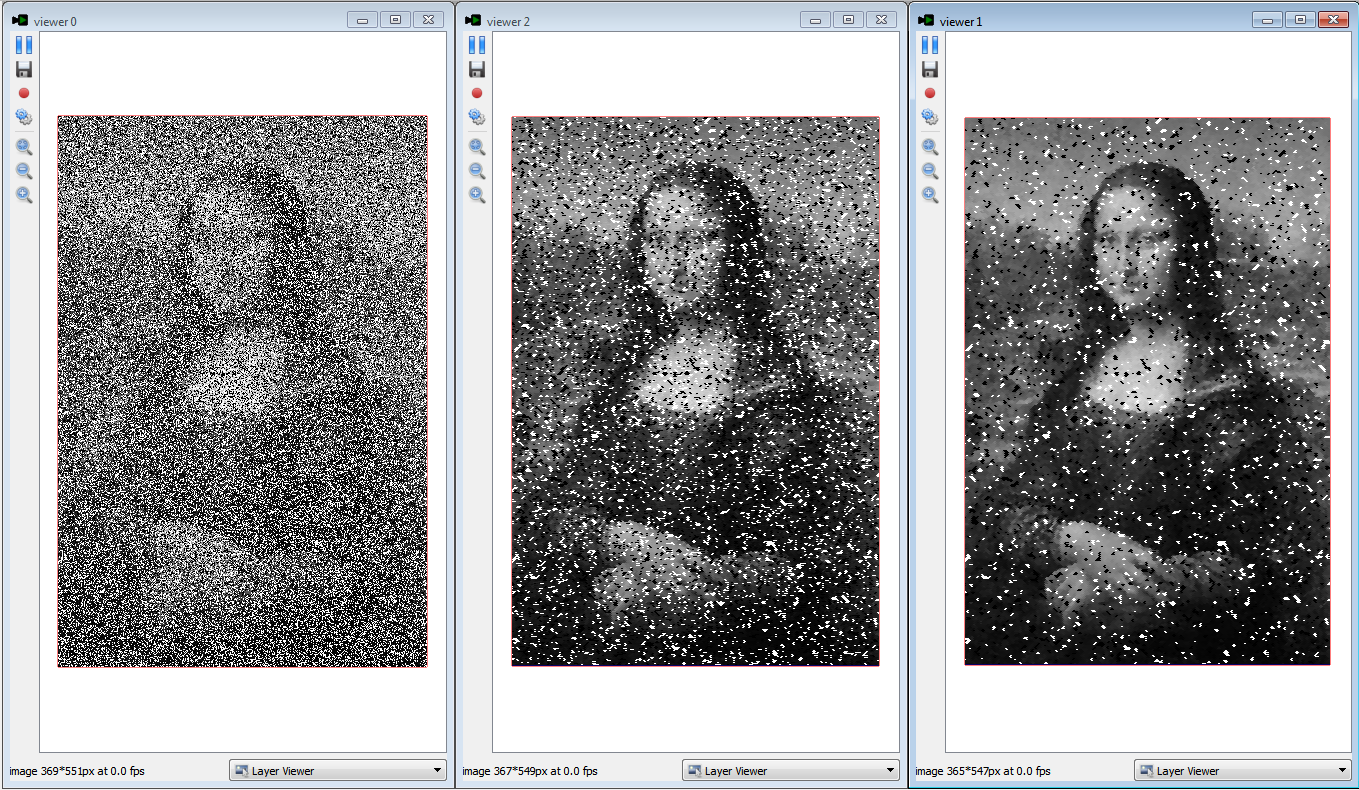
\includegraphics[width=10cm]{sp1.png}
\end{figure}

\vspace{0.5cm}

\begin{figure}[!h]
\centering
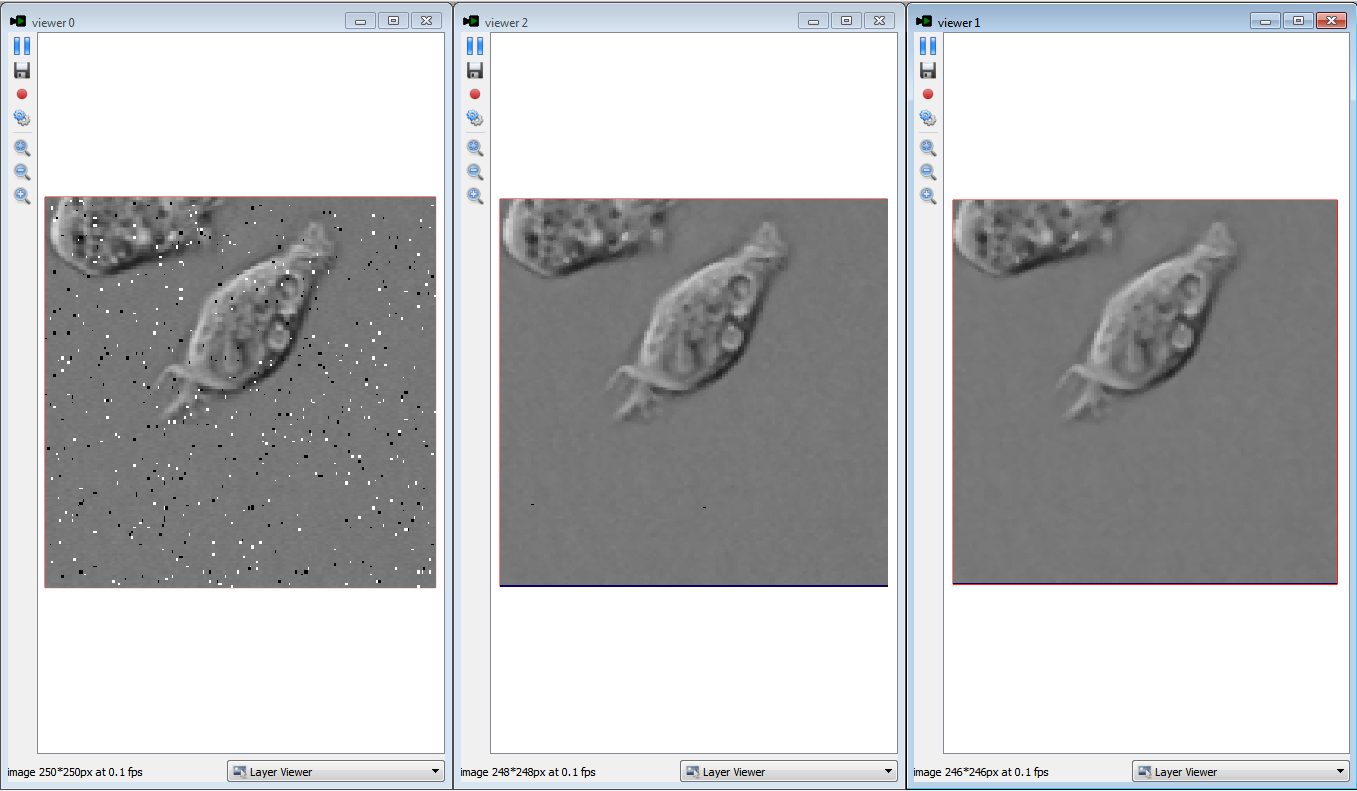
\includegraphics[width=10cm]{sp2.png}
\end{figure}

\newpage

\section*{Properties}
\properties{
enable & bool & Enable the processing \\ 
}

\vspace{1cm}

\section*{Constants}

\constants{
LINE\_WIDTH\_MAX & Maximum line size of the image : 1280 pixels  \\ 
CLK\_PROC\_FREQ & Frequency clock of the process \\
IN\_SIZE & Size of the input flow : 1 byte \\
OUT\_SIZE & Size of the output flow : 1 byte  \\
}

\vspace{0.5cm}

\section*{Equivalence}
\subsection*{Matlab}

\lstset{language=Matlab}
\begin{lstlisting}
I; % noised image
I_denoised = medfilt2(I)

\end{lstlisting}

\url{https://fr.mathworks.com/help/images/ref/medfilt2.html}

\vspace{0.5cm}
\newpage
\section*{Mathematical formalism}

Let's take a 3-by-3 pixels sliding window.  Let's sort them in ascending order. The new value of the output pixel is the central pixel value in the table of the ordered pixels.\\

Example :\\

The 3-by-3 pixels sliding window with the values of all pixels. The corrupted pixel is 251. \\

\begin{table}[h!]
\centering
\begin{tabular}{cccll}
\cline{1-3}
\multicolumn{1}{|c|}{125} & \multicolumn{1}{c|}{136} & \multicolumn{1}{c|}{127} &  &  \\ \cline{1-3}
\multicolumn{1}{|c|}{114} & \multicolumn{1}{c|}{251} & \multicolumn{1}{c|}{117} &  &  \\ \cline{1-3}
\multicolumn{1}{|c|}{121} & \multicolumn{1}{c|}{124} & \multicolumn{1}{c|}{126} &  &  \\ \cline{1-3}
\multicolumn{1}{l}{}      & \multicolumn{1}{l}{}     & \multicolumn{1}{l}{}     &  & 
\end{tabular}
\end{table}

After sorted all the pixels, the new value of the output pixel is 125. 


\begin{table}[h!]
\centering
\begin{tabular}{cclllllcll}
\cline{1-9}
\multicolumn{1}{|c|}{114} & \multicolumn{1}{c|}{117} & \multicolumn{1}{l|}{121} & \multicolumn{1}{l|}{124} & \multicolumn{1}{l|}{\textbf{125}} & \multicolumn{1}{l|}{126} & \multicolumn{1}{l|}{127} & \multicolumn{1}{c|}{136} & \multicolumn{1}{l|}{251} &  \\ \cline{1-9}
                          &                          &                          &                          &                                   &                          &                          &                          &                          &  \\
                          &                          &                          &                          &                                   &                          &                          &                          &                          &  \\
\multicolumn{1}{l}{}      & \multicolumn{1}{l}{}     &                          &                          &                                   &                          &                          & \multicolumn{1}{l}{}     &                          & 
\end{tabular}
\end{table}



\end{document}